\documentclass[reprint]{revtex4-1}
\usepackage{amsmath,amssymb}
\usepackage{graphicx}
\usepackage{cleveref}
\usepackage{circuitikz}
\usepackage{standalone}

\begin{document}
\title{Ignition and Extinction Characteristics of a Capacitively Coupled Plasma}
\author{Daniel Underwood}
\date{\today}

\begin{abstract}

\end{abstract}
\maketitle

\section{Introduction}
Plasmas are quasineutral substances consisting of ionized atoms and the electrons removed from those atoms. Due to the quasineutral nature of plasmas, electromagnetic fields outside of the plasma are negligible while the internal fields are extremely complex. While rather rare on Earth, plasmas are ubiquitous throughout the rest of the universe \cite{F.F.Chen1989}.

In our experiment, we continue the previous work of Mann and Morton \cite{Mann2015} by generating an RF signal between two electrodes, which creates a capacitively coupled plasma (CCP) between the plates with a Debye sheath at the plates, as shown in \cref{fig:plasma-sheath}.

In this paper, we will examine the equipment and errors in our experimental setup, present the results we have collected, discuss those results, and conclude with final thoughts and direction for future work.

\begin{figure}[h]
\includegraphics[width=\columnwidth]{../resources/plasma-sheath.png}
\caption{(Color Online) Capacitor plates and Debye sheath}
\label{fig:plasma-sheath}
\end{figure}

\section{Methods}

The plasma was generated within a vacuum chamber at a pressure on the order of $10^{-1}\:\rm{Torr}$ as measured by a Granville Phillips Convectron vacuum gauge. Plasma was generated by applying an RF signal between two plates separated by a distance of $8.6 \pm 0.1\:\rm{cm}$ using the plastic cup that is partially seen in \cref{fig:plasma-sheath}. The RF signal was generated by a Dressler Cesar RF Power Generator $13.56\:\rm{MHz}$ $300\:\rm{W}$ attached to an ENI Automatic Matching Network to account for reflected signals. This setup creates a capacitively coupled plasma (CCP) \cite{physics-radio-frequency}, as shown in \cref{fig:plasma-chamber-diagram}. This setup creates a plasma between the capacitor plates with Debye sheaths at the plates, as shown in \cref{fig:plasma-sheath}.  A Tektronic TDS 1002 oscilloscope was used to measure the voltage between the two plates with a 100X probe.

\begin{figure}
\includestandalone{plasma-chamber-diagram}
\caption{Plasma Chamber Setup}
\label{fig:plasma-chamber-diagram}
\end{figure}

Data was recorded manually and statistical uncertainties were taken to be the maximum change from the mean value over a two second interval. It should be noted that this is likely an overestimation of error as it is the range rather than the standard deviation of the data; this could result in errors in data analysis and overfitting of the data. There were also systematic errors in our data with a $10^{-4}\:\rm{T}$ resolution on the pressure gauge and a $2.56\:\rm{V}$ resolution in the voltage measurements. It was not necessary in this case to include the error by the power supply since the only values of interest are read at the oscilloscope, but it will likely be important for future experiments. Both of these are negligible compared to the collected statistical uncertainties except in the cases where statistical uncertainties were not obtained.

The experimental procedure was to first pump the target chamber to a vacuum of $10^{-1}\:\rm{T}$ and then apply power between the plates until a plasma ignites. At the ignition of the plasma, we collect the ignition voltage at ignition and then the equilibrium voltage once the voltage drops due to a change in properties of the material between the plates, which is now a plasma rather than a gas and thus has different electrical properties, causing the drop in voltage. The equilibrium voltage is of some interest, but is now analyzed in this paper. After the voltage drops and equilibrium voltage is taken, we decrease the power delivered by the power supply at a rate of approximately $1\:\rm{W}$ per second until the illuminated Debye sheath disappears; at this point, we collect the extinction voltage of the plasma.

The intention was to analyze the collected data in the form of a Paschen curve with the form given in \cref{eqn:paschen-curve}.

\begin{equation}
V_B = \frac{B p d}{\ln{\left( A p d \right)} - \ln{\left[ \ln{\left( 1 + \gamma_{\rm{se}}^{-1} \right)} \right]}}
\label{eqn:paschen-curve}
\end{equation}

where $V_B$ is the breakdown voltage, which we refer to as the ignition voltage, $p$ is the pressure, $d$ is the distance between the plates, $A$ and $B$ are fit parameters which are related to the saturation ionization of the gas and excitation and ionization energies, respectively, and $\gamma_{\rm{se}}$ is the secondary electron emission coefficient at the cathode \cite{Lieberman2005}.

Unfortunately, as discussed in later sections, our data was not able to be analyzed with the model due to fundamental discrepancies of the data and that of a Paschen curve.

\section{Results}

As can be seen in \cref{fig:ignition-extinction}, our collected ignition voltages do not follow the same pattern as expected by Paschen's Law. The largest evidence of this is the negative curvature that is seen in at the higher pressures -- Pachen's Law produces a curve with exclusively positive curvature. The other clear difference from Paschen's Law is that we do not find a sharp increase at lower pressures.

\begin{figure}[h]
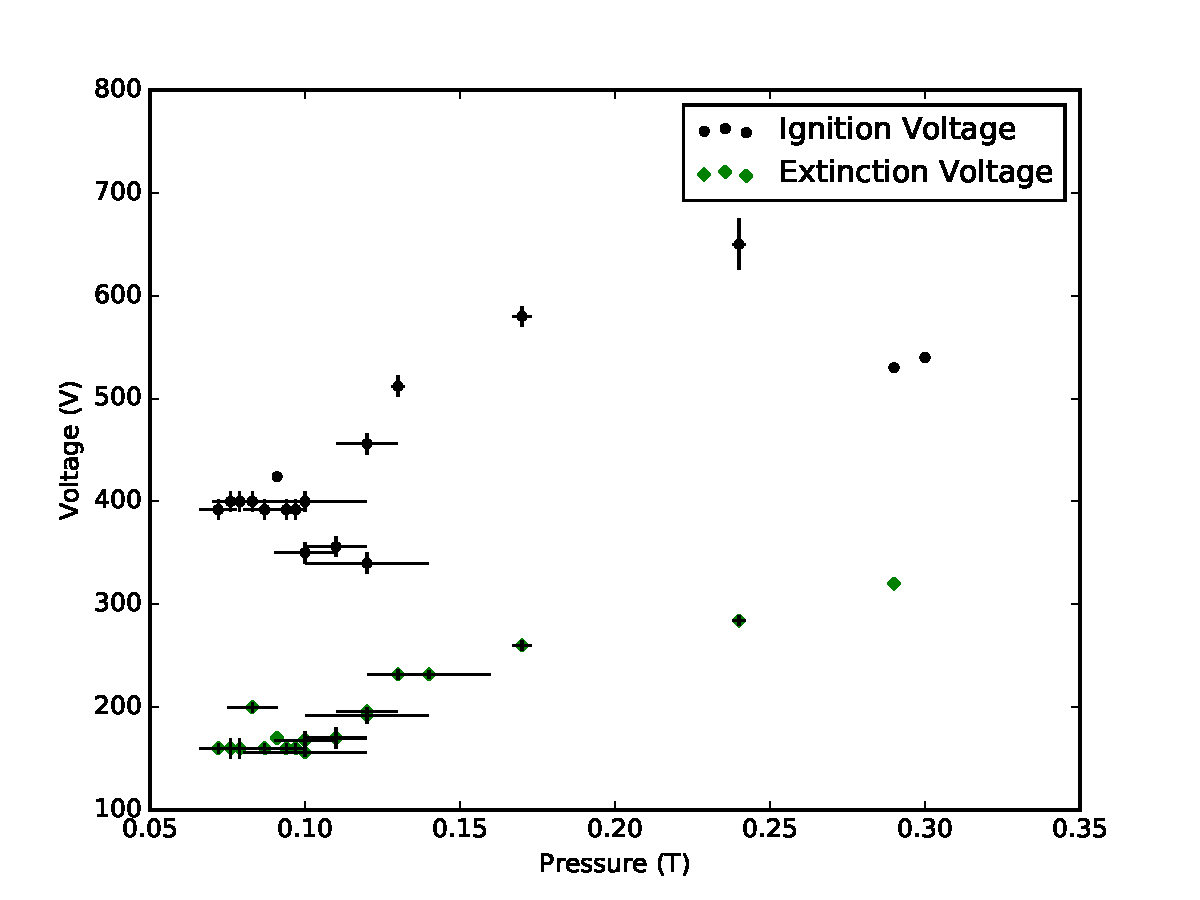
\includegraphics[width=\columnwidth]{../resources/ignition-extinction.pdf}
\caption{(Color Online) Collected ignition, equilibrium, and extinction voltage}
\label{fig:ignition-extinction}
\end{figure}

An interesting thing to note of \cref{fig:ignition-extinction} is that our collected extinction voltages follow a trend very similar to that of the ignition voltages.

\section{Discussion}



\section{Conclusion}

In the context of an educational laboratory, our experiment may be improved by continually taking measurements of the power and voltage in order to obtain the information necessary to have an IV curve for the plasma and subsequently extract IV characteristics from the plasma. In addition to our setup of a capacitively coupled plasma,  the equipment may be used to generate an inductively coupled plasma by replacing the electrode plates with a solenoid and modifying the vacuum system to pump along the axis of the solenoid, as described in \cite{physics-radio-frequency,Jiayin2010}.

\bibliography{plasma-iv-characteristics}

\end{document}